\PassOptionsToPackage{unicode}{hyperref}
\PassOptionsToPackage{hyphens}{url}
%
\documentclass[superscriptaddress, 12pt]{revtex4-2}%twocolumn
\usepackage{amsmath,amssymb}
\usepackage{iftex}
% Use upquote if available, for straight quotes in verbatim environments
\usepackage{xcolor}
\usepackage{subcaption}
%\usepackage{longtable}
\usepackage{booktabs,array}
\usepackage{multirow}
\usepackage{calc} % for calculating minipage widths
% Correct order of tables after \paragraph or \subparagraph
\usepackage{etoolbox}
\usepackage{footnote}
\usepackage{graphicx}
\usepackage{bookmark}
%\usepackage{babel}
\IfFileExists{xurl.sty}{\usepackage{xurl}}{} % add URL line breaks if available
\urlstyle{same}
\hypersetup{
  hidelinks,
  pdfcreator={LaTeX via pandoc}}
\usepackage{textgreek}
\usepackage{makecell}
\usepackage{multirow}
\usepackage{booktabs}
\usepackage[LGR,T1]{fontenc}
\usepackage[utf8x]{inputenc}
\usepackage{textalpha}
\usepackage{ulem}
\usepackage{textcomp}
\date{}


\begin{document}

\title{Influence of partial occupancy on the elastic tensor for FeCr \textsigma - phase.}

\author{Mariano Forti} \email{mariano.forti@icams.rub.de}
\affiliation{Interdisciplinary cetre for advanced materials simulations (ICAMS), Ruhr Universität Bochum, Germany}

\author{Thomas Hammerschmidt} \email{}
\affiliation{Interdisciplinary cetre for advanced materials simulations (ICAMS), Ruhr Universität Bochum, Germany}

\author{Guillaume Laplanche} \email{}
\affiliation{Ruhr Universität Bochum}


\maketitle

\section{Introduction}

The Fe-Cr system is an important alloy system with applications in structural and high-temperature environments.
The \textsigma-phase can form at Cr concentrations between 45 and 50\%at and temperatures ranging from 550 to 800\textdegree ~\cite{laplanche_phase_2018} significantly influencing the mechanical properties.
Specifically, \textsigma-phase precipitation contributes to embrittlement and reduces corrosion resistance {\color{red}  [ref 2 detrimental sigma] }.
The \textsigma-phase unit cell is shown in \autoref{fig:sigmaUnitCell}.
This is an intermetallic compound with a tetragonal structure (space group P4\textsubscript{2}/mnm) and exhibits complex atomic arrangements due to site-specific partial occupancies.
Understanding its properties is essential for predicting its mechanical behavior and phase stability.
There are different approaches to similar problems in atomistic simulations, based for instance on Density Functional Theory (DFT).
Vesti et. al. ~\cite{vesti_ab-initio_2023} utilize a full sublattice model later averaged under an ideal mixing approximation to interpolate the properties of a W-Re \textsigma phase.
Kabliman et. al. ~\cite{kabliman_ab_2012} use a mean field approximation to study several properties of the \textsigma phase in other binary systems, also based on full occupancy of the sublattices.
This assumption may overlook local atomic configuration effects.
In this work, we investigate how explicit consideration of partial occupancy influences the elastic properties of the \textsigma-phase through first-principles calculations.
We focus on a Fe16Cr14 unit cell which can be modelled with nominal and on-site compositions in agreement with experimental observations.

\begin{figure}
  \subcaptionbox{\protect\label{fig:sigmaUnitCell}}{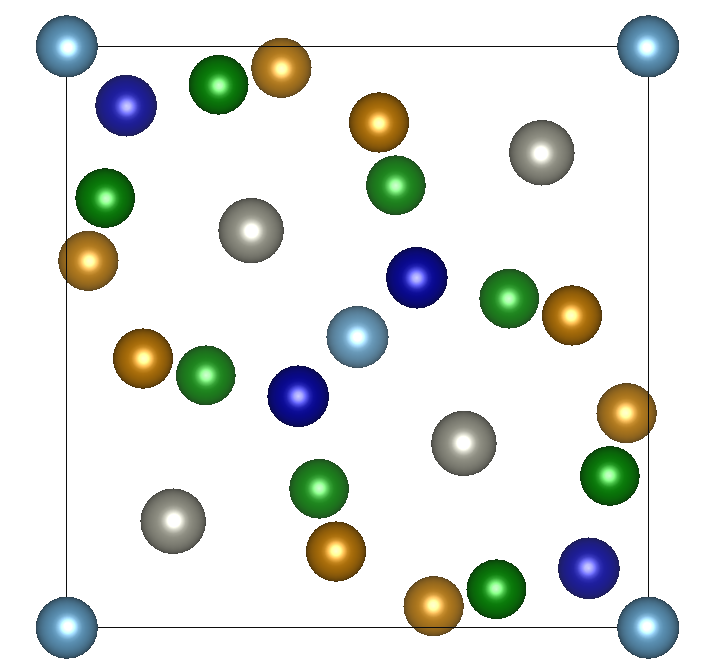
\includegraphics[height=4cm]{Figure_SigmaPhase001.png}}
  \caption{\protect\label{fig:introduction}
    (\subref{fig:sigmaUnitCell}) (001) view of the σ phase unit cell.
    Wyckoff sites are encoded in colors: 2a is light blue,
    4f in grey, 8i in green, 8i' in gold, 8j in blue.
  }
\end{figure}

\section{Methodology}

We employ first-principles DFT calculations to determine the elastic constants of the Fe-Cr \textsigma-phase at a nominal composition of Fe\textsubscript{16}Cr\textsubscript{14} (48\%at. Cr).
These calculations are conducted using the Vienna Ab initio Simulation Package (VASP) ~\cite{Hafner_vasp}, utilizing the Perdew-Burke-Ernzerhof (PBE) ~\cite{Perdew1996} exchange-correlation functional and the Projector Augmented Wave (PAW) method ~\cite{Bloch1994, kresse_ultrasoft_1999}.
The elastic tensor is derived from stress-strain relationships obtained via energy-strain calculations.


\paragraph{Full occupancy}

First, we calculate the properties of the \textsigma-phase using a full sublattice model.
This means, that the lattice positions of a WS are occupied either by Cr or Fe.
We calculate formation enthalpies and elastic constants for all the possible configurations spanning the full composition range.

\paragraph{Partial occupancy} To capture the impact of atomic disorder, we explicitly explore all possible atomic arrangements within the \textsigma-phase unit cell, incorporating experimentally reported partial occupancies of Wyckoff sites by Yakel~\cite{yakel_atom_1983} as reproduced in \autoref{fig:ExptPartialOccupancies}.  
A random distribution in the different sublattices could be modelled for instance by a special quasirandom structure [SQS ref] but  this would require a big unit cell to generate a meaningful representation of such atomic distributions.  
In addition to this, the measured composition of the 2a site (< 0.5 atom per unit cell) would require a bigger unit cell to model it accurately.
In order to keep the size of the simulation cell to one unit cell, we consider two approximations to the partial occupancies, in both cases disregarding Cr occupation in site 2a and rounding occupancies to integer numbers.  
A first model, \autoref{fig:PartialOccupanciesA}, keeps one Fe atom in the site 4f and 1 Cr atom in site 8i'.  
In this condition, the total number of possible configurations is $ 1 \times 4 \times \binom{8}{3}\times \binom{8}{1} \times \binom {8}{3} \approx 100k $, which are too many to consider DFT calculations of a significant sample. 
We name this model 2\_A3B\_A5B3\_AB7\_A5B3.  
A second model, \autoref{fig:PartialOccupanciesb}, keeps the same number of atoms in the 8i and 8j sites, while transferring the Cr atom from 8i' to 4f.  
We call this other model B2\_A3B2\_A5B3\_B8\_A5B3. 
This reduces the number of possible configurations to $1 \times 1 \times \binom{8}{3}\times 1\times\binom {8}{3} = 3136$.~
%, which is a more manageable number of configurations. 
A subset of 25 representative configurations of each model is selected for detailed elastic constant calculations. ~\cite{golesorkhtabar_elastic_2013}.

\begin{figure}
  \subcaptionbox{\protect\label{fig:ExptPartialOccupancies}}{\includegraphics[height=4cm]{example-image-a}}
  \subcaptionbox{\protect\label{fig:PartialOccupanciesA}}{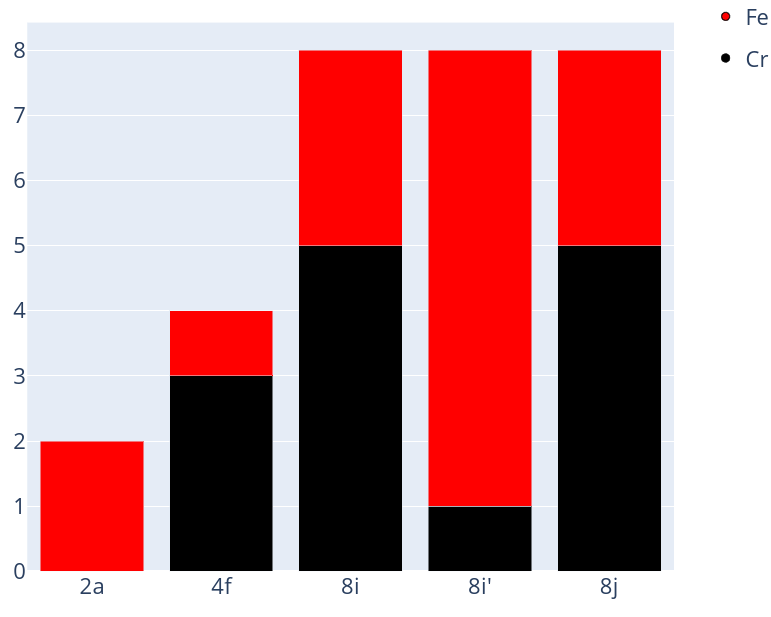
\includegraphics[height=4cm]{Figure_SigmaPhaseModelledPartialOccupancies_II.png}}
  \subcaptionbox{\protect\label{fig:PartialOccupanciesb}}{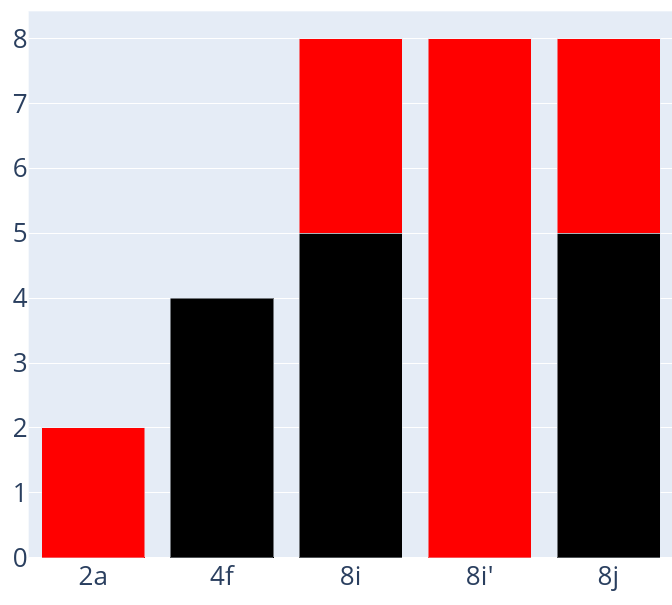
\includegraphics[height=4cm]{Figure_SigmaPhaseModelledPartialOccupancies.png}}

  \caption{\protect\label{fig:PartialOccupancies}
    (\subref{fig:ExptPartialOccupancies}) 
    (001) view of the σ phase unit cell.
    Wyckoff sites are encoded in colors: 2a is light blue,
    4f in grey, 8i in green, 8i' in gold, 8j in blue.
    (\subref{fig:PartialOccupanciesA}) 
    First model of unit cell with partial occupancy, model B2\_A3B\_A5B3\_AB7\_A5B3.
    (\subref{fig:PartialOccupanciesB}) 
    Further simplified model B2\_A3B2\_A5B3\_8B\_A5B3.
  }

\end{figure}

\section{Results}

In a full sublattice model, the Fe-Cr \textsigma phase has a tetragonal unit cell in the space group P4\textsubscript{2}/mnm in the entire composition range.  
Our results show that partial occupancy disrupts unit cell symmetry, significantly affecting the mechanical response of the \textsigma-phase.  
Using \textit{spglib}\marginpar{\tiny spglib ref!} as implemented in \textit{ase} \marginpar{\tiny ase ref!}, we find that even before full optimization of the unit cell, the only decoration of the lattice  sites according to the partial occupancy breaks the tetragonal symmetry of the sigma phase.  
\marginpar{\tiny would it be possible that occupancy in 2a recovers symmetry somehow?}
Upon decoration, all the configurations acquire a triclinic unit cell with space group P1. 
The cell vector lengths and angles of the triclinic cells are shown in \autoref{fig:Symmetry_angles_caratio} for all the configurations.  
Although small, the introduced structural variations might affect the mechanical properties of the \textsigma -phase. 

\paragraph{phase stability}

\autoref{fig:OccupancyEffect} shows the calculated convex hull for the full occupancy samples and both models with
partial occupancy. 
The formation enthalpies of the \textsigma~phase are possitive for all compositions, which indicate that it it could be stabilized by entropy contributions. 
However, at the composition of interest, introducing partial occupancy stabilizes the phase as several samples have a formation enthalpy below the tie-line of the full-occupancy convex hull. 

\paragraph{Elastic constants}

Due to the low symmetry, the elastic tensor of the triclinic unit cell has 22 independent components, and their determination is computationally much more demanding than the full occupancy cases, requiring a larger number of DFT calculations.
Finally, in \autoref{fig:VRHelastic} we report the changes in the VRH averaged elastic moduli with nominal composition and fractional occupation of the sublattices.
We observe a slight stiffening of the compound for increasing Cr content, which is consistent with experimental findings.

\begin{figure}
  \subcaptionbox{\protect\label{fig:Symmetry_angles_caratio}}{\includegraphics[height=4cm]{example-image-a}}
  \caption{\protect\label{fig:SymmetryConsiderations}
    (\subref{fig:Symmetry_angles_caratio}) 
    Distribution of angles and c/a ratio for full occupancies and models with partial occupancies. 
  }
\end{figure}

\begin{figure}
 \subcaptionbox{\protect\label{fig:ConvexHull0k}}{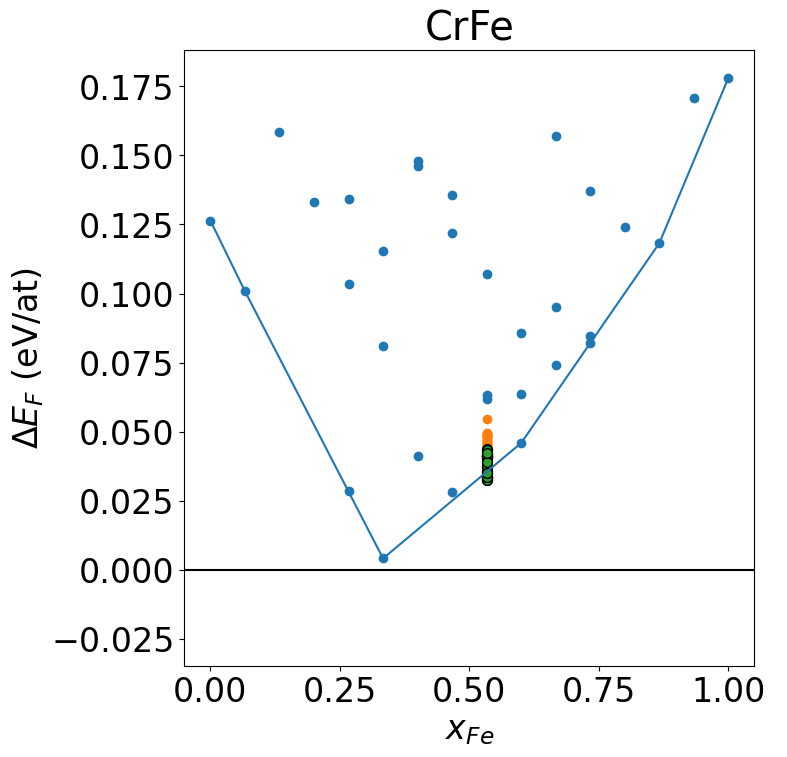
\includegraphics[height=4cm]{Figure_FeCrSigmaConvexHull.png}}
 \subcaptionbox{\protect\label{fig:VRHelastic}}{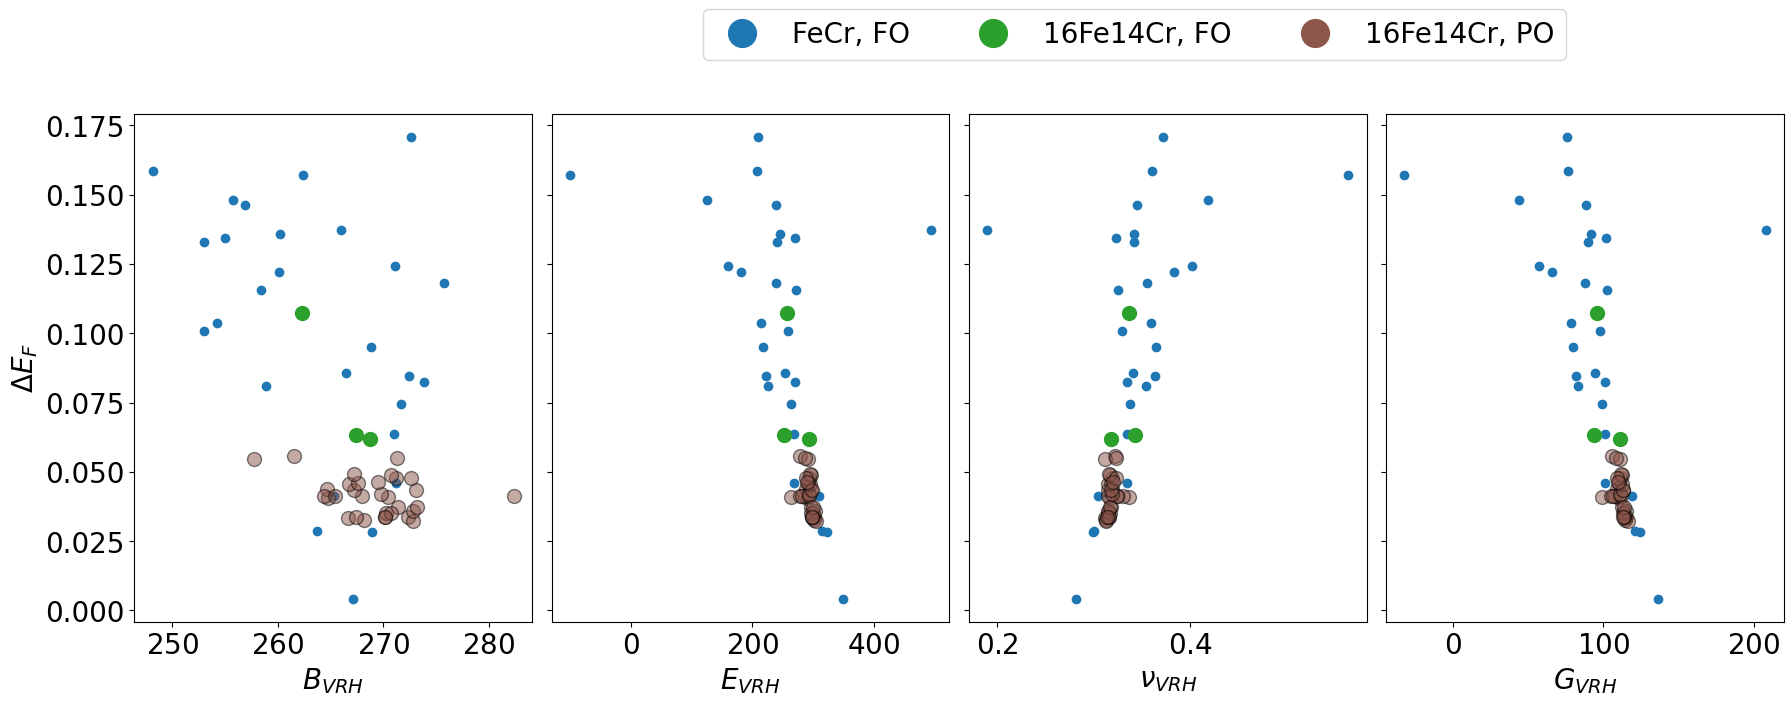
\includegraphics[height=4.5cm]{Figure_VRHAVerages.png}}
 \caption{\protect\label{fig:OccupancyEffect}
   Effect of occupancy on the stability and properties of the Fe16Cr14 \textsigma-phase.
   (\subref{fig:ConvexHull0k}) Effect on formation enthalpy at 0K.
   (\subref{fig:ConvexHull0k}) Effect on VRH averaged elastic moduli.
 }

\end{figure}

\section{Conclusion}
In this work, we are presenting a methodical study of the effects of partial occupancy in the properties of the \textsigma phase of the FeCr system.
For the first time, the properties of this phase are calculated taking into account the experimentally observed partial occupancies.
We demonstrate that partial occupancy significantly influences the mechanical response of the \textsigma-phase, which cannot be captured by the traditional full sublattice models.
Our results provide new insights into the mechanical behavior of the Fe-Cr \textsigma-phase and highlight the importance of considering partial occupancy in theoretical models.


\section{full occupancies}

\section{selection of working alloy}
final long term goal is CrMnFeCoNi (order by atomic number).
We select the easiest binary with $\sigma$ phase.
We select 16Fe14Fe because it was close to the experimental 50\%Fe and it is easy to distribute between the sublattices.
show experimental partial occupancies, and the modelled distributions.
(there are slides)
explaining breaking of symmetry by partial occupancies with figures.


\bibliographystyle{naturemag} \bibliography{main.bib}

\end{document}
